\begin{figure*}[t]
\centering
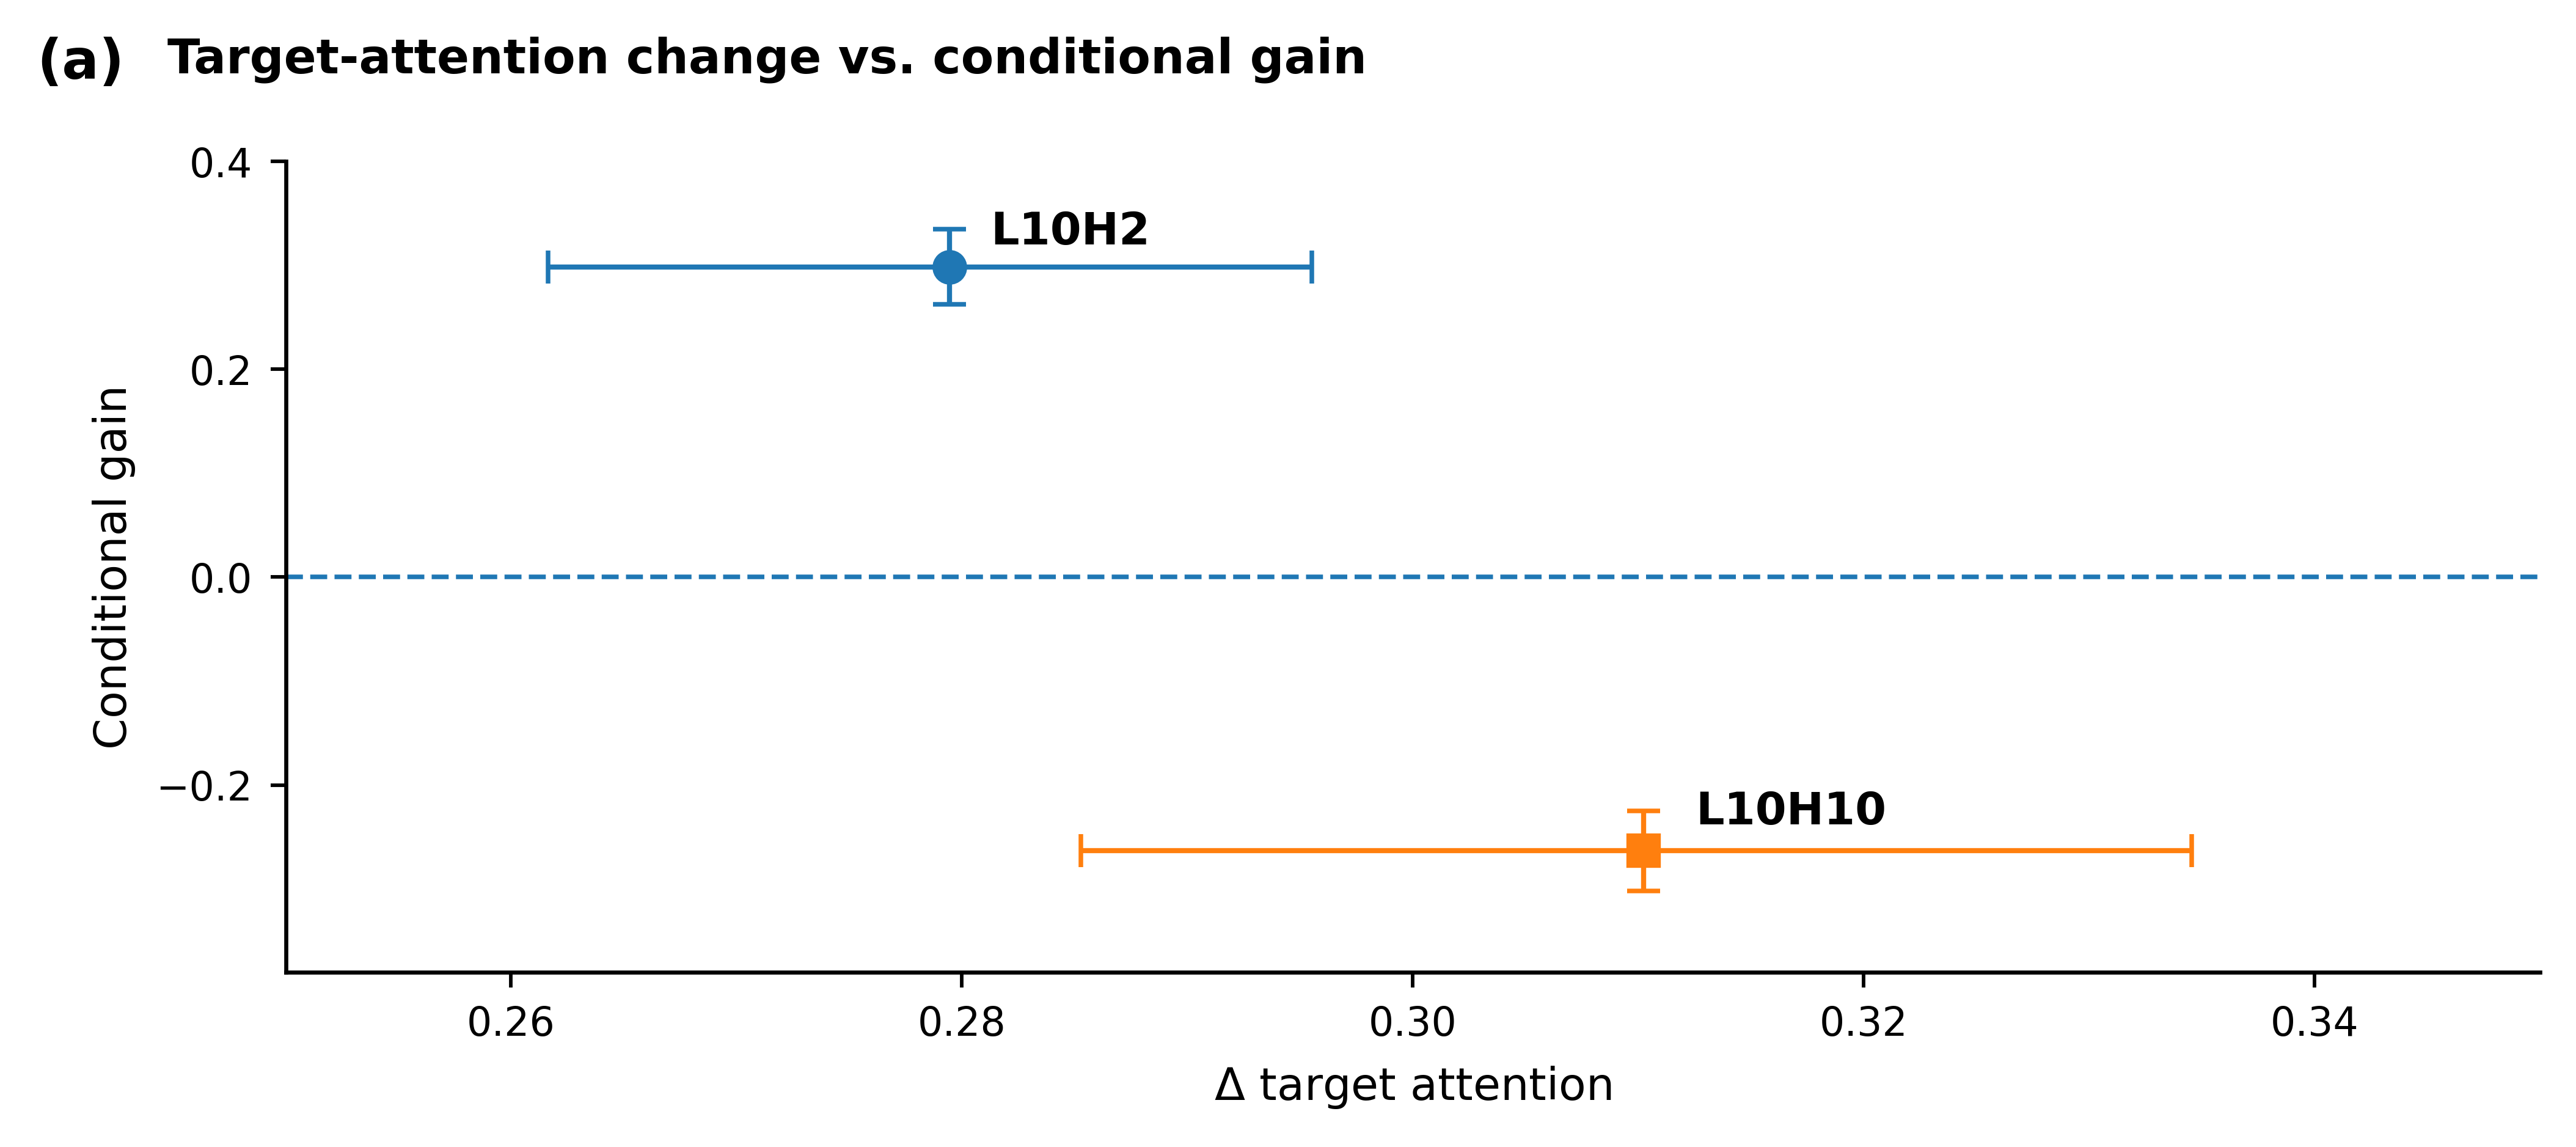
\includegraphics[width=0.95\textwidth]{figures/Fig4a.png}
\caption{\textbf{Target-attention adaptation is not sufficient for positive functional recruitment in GPT-2 IOI.}
(a) L10H2 and L10H10 both increase attention to the indirect-object target after ablation of the canonical primary Name Movers, but their conditional gains have opposite signs: L10H2 becomes more causally useful whereas L10H10 becomes less useful on the broad canonical distribution.
Points are exact balanced means; horizontal and vertical intervals are hierarchical 95\% bootstrap confidence intervals over the canonical template design.}
\label{fig:gpt2-attention-recruitment}
\end{figure*}
